\chapter{Resultados numéricos}

Neste capítulo, apresenta-se o método numérico de solução do modelo apresentado neste trabalho, os recursos computacionais utilizados, os sistemas que foram testados e as soluções numéricas obtidas. 


Conforme apresentado nos capítulos anteriores, o modelo proposto nesta tese possui duas funções objetivo. A primeira busca minimizar o valor presente líquido dos custos de investimento, manutenção, perdas técnicas e com geração de energia ($c^{TPV}$). A segunda função objetivo busca maximizar a injeção de corrente considerada "segura"\; em quaisquer dos nós do sistema de distribuição ($J^{HC}_t$).

Entretanto, um dos objetivos desta tese é analisar os aspectos que relacionam o valor de \ac{HC} com os custos do \ac{PESD}. Portanto é necessário observar como as alterações no custo do \ac{PESD} impactam o valor de \ac{HC}. Para tal análise, foi escolhido identificar alguns dos \textit{pontos ótimos da Fronteira de Pareto}\footnote{Neste capítulo utiliza-se os seguintes conceitos como sinônimos: ponto ótimo da Fronteira de Pareto, solução ótima da Fronteira de Pareto, solução Pareto-ótima, ponto Pareto-ótimo} do modelo apresentado.

Para os leitores que não estão familiarizados com o conceito de Fronteira de Pareto em otimização ou com técnicas de solução de modelos multi-objetivos, recomenda-se a leitura do artigo de \citeonline{oliveira2010multiobjective}. Porém, de forma geral e resumida, os pontos ótimos da fronteira de Pareto de um modelo bi-objetivo linear inteiro misto, são soluções que satisfazem ambas as funções objetivo e que não há nenhuma outra solução que as \textit{domine}, ou seja, não há outra solução que melhore ainda mais uma das funções objetivos, sem necessariamente degradar a outra. 


\section{Método numérico de resolução}

Sabe-se que comumente é computacionalmente inviável (mesmo que teoricamente possível), obter todas as soluções Pareto-ótimas de modelos complexos. Portanto, métodos numéricos são aplicados para se obter as soluções numéricas Pareto-ótima destes modelos. Dentre várias opções possíveis, foi escolhido o método Hierárquico (também conhecido como Lexicográfico) em conjunto com o método $\epsilon$-restrito (também conhecido como \textit{trade-off}) para a busca de soluções Pareto-ótima do modelo apresentado. Detalhes teóricos, numéricos e específicos de cada método fogem do escopo desta tese, recomenda-se novamente o artigo de \citeonline{oliveira2010multiobjective} para uma introdução ao tema.

No modelo hierárquico, definiu-se que \ac{HC} possui uma hierarquia maior que o os custos do \ac{PESD}, ou seja, na resolução do modelo hierárquico, resolve-se primeiro a função objetivo de \ac{HC} e então fixa-se o valor de \ac{HC} e resolve-se o modelo para a função objetivo de custos do \ac{PESD}.

A figura \ref{fig:method} descreve a implementação destes métodos e como foi feita a integração entre o método Hierárquico com o $\epsilon$-restrito. Os parâmetros de entrada do método utilizado dependem de um valor inicial de $c^{TPV}$ (representada na figura \ref{fig:method} como $c^{TPV - HC}$) e de um valor de $\epsilon$. Estes valores são utilizados para decrementar o limite máximo de $c^{TPV}$ do modelo hierárquico, configurando assim, como um método $\epsilon$-restrito. Nesta abordagem, sugere-se um valor inicial de $c^{TPV - HC}$ grande o suficiente para que na primeira iteração o valor da função objetivo de \ac{HC} seja a maior possível. Nesta tese, utilizou-se $\epsilon = 450$ e $c^{TPV - HC} = 10^{10}$ como entrada para todas as análises.

\begin{figure}[ht]
 	\centering
    \caption{Abordagem para a resolução do modelo bi-objetivo.}
        \begin{tikzpicture}[node distance=2cm]
        \node (start) [startstop] {Início};
        \node (in1) [io, below of=start, xshift=-2.5cm] {Valor inicial de \\ $c^{TPV - HC}$};
        \node (in2) [io, right of=in1, xshift=2.5cm] {Valor de $\epsilon$};
        \node (pro1) [process, right of=start, xshift=5cm] {Resolva o modelo apenas \\ para $c^{TPV}$};
        \node (pro2) [process, below of=pro1] {$c^{TPV - MIN} \leftarrow c^{TPV}$};
        \node (dec1) [decision, below of=in2, yshift=-0.3cm] {$ c^{TPV - HC} - c^{TPV - MIN} > \epsilon$};
        \node (stop) [startstop, right of=dec1, xshift=4.5cm] {Fim};
        \node (pro3) [process, below of=dec1, yshift=-0.5cm] {Adicione nova restrição\\$c^{TPV} \leq c^{TPV - HC} - \epsilon$};
        \node (pro4) [process, below of=pro3] {Resolva o modelo bi-objetivo\\hierárquico};
        \node (out1) [io, right of=pro4, xshift=3.5cm] {Salve\\a solução};
        \node (pro5) [process, left of=pro4, xshift=-3.5cm] {$c^{TPV - HC} \leftarrow c^{TPV}$};
        \node (pro6) [process, above of=pro5] {Remova a restrição\\adicionada};
        \draw [arrow] (start) --  (in1);
        \draw [arrow] (start) -- (in2);
        \draw [arrow] (start) -- (pro1);
        \draw [arrow] (pro1) -- (pro2);
        \draw [arrow] (in1) -- (dec1);
        \draw [arrow] (in2) -- (dec1);
        \draw [arrow] (pro2) -- (dec1);
        \draw [arrow] (dec1) -- node[anchor=south] {Não} (stop);
        \draw [arrow] (dec1) -- node[anchor=east] {Sim} (pro3);
        \draw [arrow] (pro3) -- (pro4);
        \draw [arrow] (pro4) -- (out1);
        \draw [arrow] (pro4) -- (pro5);
        \draw [arrow] (pro5) -- (pro6);
        \draw [arrow] (pro6) |- (dec1);
        \end{tikzpicture}\\
    Fonte: Próprio autor
    \label{fig:method}
\end{figure}

Como todo método $\epsilon$-restrito, a abordagem utilizada possui as mesmas características. Isto significa que valores muito grandes de $\epsilon$ encontrará menos soluções Pareto-ótimas e, portanto, o algoritmo finalizará mais rápido. Já valores muito pequenos de $\epsilon$ encontrará mais soluções Pareto-ótimas, porém, o algoritmo levará mais tempo para finalizar. Teoricamente, com $\epsilon$ tendendo a zero, é possível obter todas as soluções Pareto-ótimas, apesar de ser inviável computacionalmente para modelos complexos.

\section{Recursos computacionais, código fonte e dados}

A implementação e resolução do modelo bi-objetivo foi realizada em um computador Intel i5-8400 com seis núcleos de até 4 GHz, 16 GB de memória RAM DDR4. O computador utilizado executa o sistema operacional Fedora Linux 38 com kernel Linux 6.4. Não foi utilizado processamento com placa de vídeo nesta implementação.

Os modelos e a abordagem de resolução foram implementados em linguagem Julia, uma linguagem de programação livre e de código aberto projetada para atender as demandas atuais de métodos numéricos e programação científica, apresentada no trabalho de \citeonline{Julia-2017}. Foi utilizado também o pacote JuMP para modelagem de problemas de otimização matemática,  apresentado no trabalho de \citeonline{DunningHuchetteLubin2017}. Para a solução do modelo foi utilizado o \textit{solver} Gurobi \cite{gurobi} sob a abstração do pacote Gurobi.jl \cite{gurobijl} em conjunto com o pacote JuMP. As versões de cada \textit{software} são encontradas na tabela \ref{tab:list_soft}.

\begin{table}[ht]
\centering
\caption{Lista de \textit{softwares} utilizados e suas respectivas versões}
\label{tab:list_soft}
\begin{tabular}{@{}lc@{}}
\toprule
\textit{Software} & Versão   \\ \midrule
Julia                              & 1.9.3    \\
JuMP                               & 1.14.0   \\
Gurobi.jl                          & 1.0.3    \\
Gurobi                             & 10.0.2 \\ \bottomrule
\end{tabular}
\\Fonte: Próprio autor
\end{table}

A linguagem, pacotes e \textit{solver} foram escolhidos devido a familiaridade que o autor deste trabalho possui com estes \textit{softwares}, porém, este modelo pode ser implementado em qualquer \textit{solver} de preferência. 

Para a resolução do modelo hierárquico, foi utilizado a abordagem built-in do \textit{solver} Gurobi, configurando a função objetivo de \ac{HC} para prioridade 10 e a função de custos do \ac{PESD} para prioridade 1.

Com o objetivo de fomentar a reprodutibilidade e inspeção dos resultados, todo o código fonte utilizado para a implementação, tanto do modelo base \cite{modelobase}, quanto para o modelo com \ac{HC} \cite{modelocomHC}, estão disponíveis em repositórios Git sob licença Apache v2.0 (uma licença de código aberto e permissiva tanto para cópia, modificação e distribuição). 

Durante a escrita desta tese, o autor trabalha para que os modelos possam ser utilizados como pacotes Julia para serem facilmente importados em trabalhos futuros.


\subsection{Dados de sistemas de distribuição utilizados}

Para demonstrar o modelo e a abordagem proposta, foram utilizados três sistemas baseados em sistemas de distribuição amplamente conhecidos na literatura. Foi necessário realizar alterações nos dados dos sistemas da literatura pois o modelo e a abordagem proposta escalam exponencialmente com o tamanho do modelo e com a quantidade de estágios. Esta desvantagem foi observada após vários meses de implementação, testes e melhoria do código para que fosse possível obter os resultados apresentados nesta tese. Vale ressaltar que as alterações realizadas foram principalmente na quantidade de estágios e nos limites de investimentos. Todos os parâmetros dos modelos podem ser encontrados no repositório Git em \cite{modelocomHC}\footnote{Foi decido não adicionar os dados das redes utilizadas no corpo de texto desta tese, pois, o autor acredita que qualquer forma de reprodução e inspeção das informações contidas neste texto é melhor realizada com o acesso direto aos dados eletrônicos utilizados. Observa-se que a abordagem de prover acesso aos dados diretamente de forma eletrônica é a mesma utilizada em muitos trabalhos publicados atualmente na área de planejamento, veja \citeonline{Confiability_Munoz} e \citeonline{MunozDelgado2015}.}, para serem inspecionados em caso de dúvidas.

O primeiro é o sistema de distribuição de 24 nós que opera a 20 kV, com três estágios de 1 ano cada e uma demanda total máxima de 46,85 MVA no último estágio. Este sistema é baseado no sistema de 24 nós encontrado no trabalho de  \citeonline{MunozDelgado2015}.

O segundo é o sistema de distribuição de 54 nós que opera a 13.5 kV, com um estágio de 3 anos e uma demanda total máxima de 72 MVA. Este sistema é baseado no sistema de 54 nós encontrado no trabalho de  \citeonline{Confiability_Munoz}.

O terceiro é o sistema de distribuição de 138 nós que opera a 13.8 kV, com um estágio de 10 anos e uma demanda total máxima de 38,13 MVA. Este sistema é baseado no sistema de 138 nós encontrado no trabalho de \citeonline{MunozDelgado2015}.





\section{Resultados para o sistema de 24 nós}

Para o sistema de 24 nós, foram realizados três cenários de análise, o primeiro considerando apenas o \ac{HC} para geração distribuída, o segundo considerando o \ac{HC} apenas para veículos elétricos ou novas cargas e o terceiro considerando ambos. Estes cenários podem ser avaliados com a alteração dos parâmetros $\alpha^{HC}$, conforme descrito na seção anterior.

Ao executar a resolução do modelo bi-objetivo para apenas geração distribuída, obteve-se apenas duas soluções, uma com valor de 784 kVA de \ac{HC} e 250,33 milhões de dólares de $c^{TPV}$ e outra com 452 kVA de \ac{HC} e 250,298 milhões de dólares de $c^{TPV}$. Por outro lado, tanto para apenas veículos elétricos ou novas cargas quanto para ambos (veículos elétricos e geradores distribuídos), foram obtidas nove soluções com uma grande variação, tanto de \ac{HC}, quanto de $c^{TPV}$. A figura \ref{fig:24_pareto} apresenta as soluções obtidas, as opções de investimentos podem ser vistas também no Apêndice \ref{sec:tab24}.

\begin{figure}[ht]
 	\centering
    \caption{24 nós -- Soluções encontradas.}
    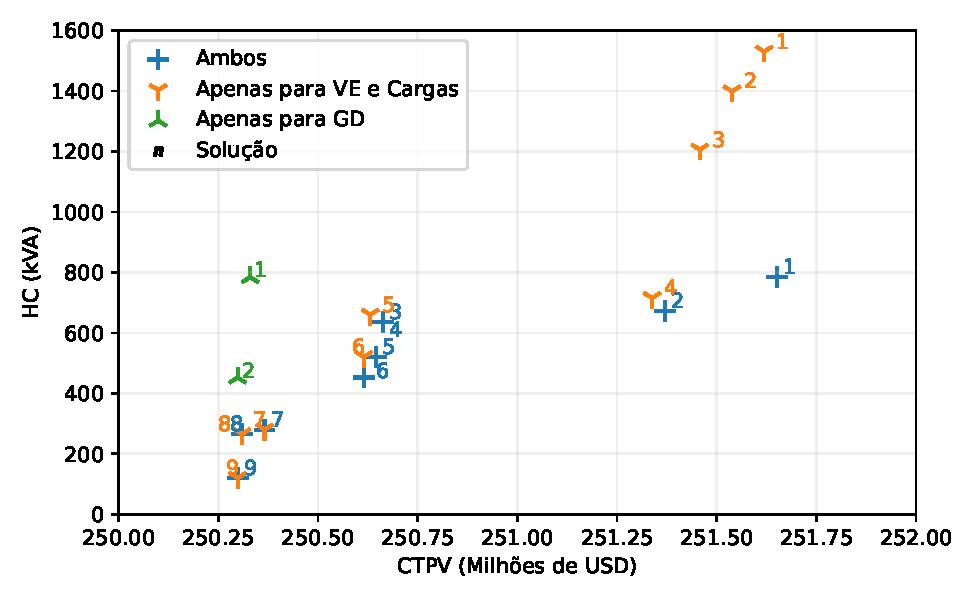
\includegraphics[width=0.8\textwidth]{cap4/resultados/24_pareto.pdf}\\
    \label{fig:24_pareto}
\end{figure}


Vale destacar como planejar o sistema de distribuição apenas visando minimizar os custos, impacta diretamente no valor de \ac{HC} do sistema de distribuição. Visando apenas custos para o cenários de ambos, chega-se a um valor de 120 kVA a um custo de 250,3 milhões de dólares. Já visando apenas \ac{HC} para o cenários de ambos, chega-se a um valor de 784 kVA a um custo de 251,65 milhões de dólares, aproximadamente uma relação de 492 kVA por milhão de dólares, em um investimento que na casa de um quarto de bilhão de dólares.


A discrepância de quantidades de soluções entre o cenário de apenas geradores distribuídos e os outros levantaram o questionamento da causa desta diferença. Inicialmente, foram testadas alterações no valor de pico das cargas e valores de cenários de carregamentos, porém, não foi encontrada nenhuma evidência que essas alterações impactaram diretamente a diferença de soluções entre os cenários avaliados. Desta forma, optou-se por investigar a fundo as soluções encontradas. A seguir, soluções pertinentes são discutidas para identificar o que impacta a relação entre \ac{HC} e $c^{TPV}$, bem como a quantidade de soluções encontradas.

\newpage
\subsection{Resultados para o sistema de 24 nós -- Apenas geração distribuída}

Como foram obtidas apenas duas soluções para o caso de apenas geração distribuída, facilmente podemos avaliar a diferença entre cada solução. Na figura \ref{fig:24_gen}, observa-se que esta diferença está relacionada apenas à localização de um gerador eólico instalado no sistema no último estágio.
Esta é a primeira evidência que a localização de geradores distribuídos podem impactar no valor de \ac{HC} em sistemas de distribuição. Porém, vale destacar que não houve diferença entre a localização de geradores distribuídos que podem ser operados pela empresa de distribuição (apresentados na figura \ref{fig:24_gen} como geradores convencionais "CX"), apenas geradores distribuídos renováveis impactaram no valor de \ac{HC} neste cenário.

Esta observação é enfatizada ao verificarmos na literatura todos os trabalhos que discutem como controlar e integrar estes tipos de geradores em sistemas de distribuição, conforme visto na seção \ref{hc_review_control_dg}.

Destaca-se também que esta observação ocorreu apenas após a adição dos cenários de geradores renováveis distribuídos (através do parâmetro $\alpha^{RW}$) no modelo base de otimização. Sem as mudanças propostas por este trabalho no modelo de \citeonline{MunozDelgado2015}, esta observação não se torna possível e o modelo retorna apenas uma solução de \ac{HC} para este cenário.
\newpage

\begin{figure}[H]
 	\centering
    \caption{24 nós -- Solução 1 e 2 para o caso de apenas GD. Em vermelho: apenas solução 1. Em verde: apenas solução 2.}
    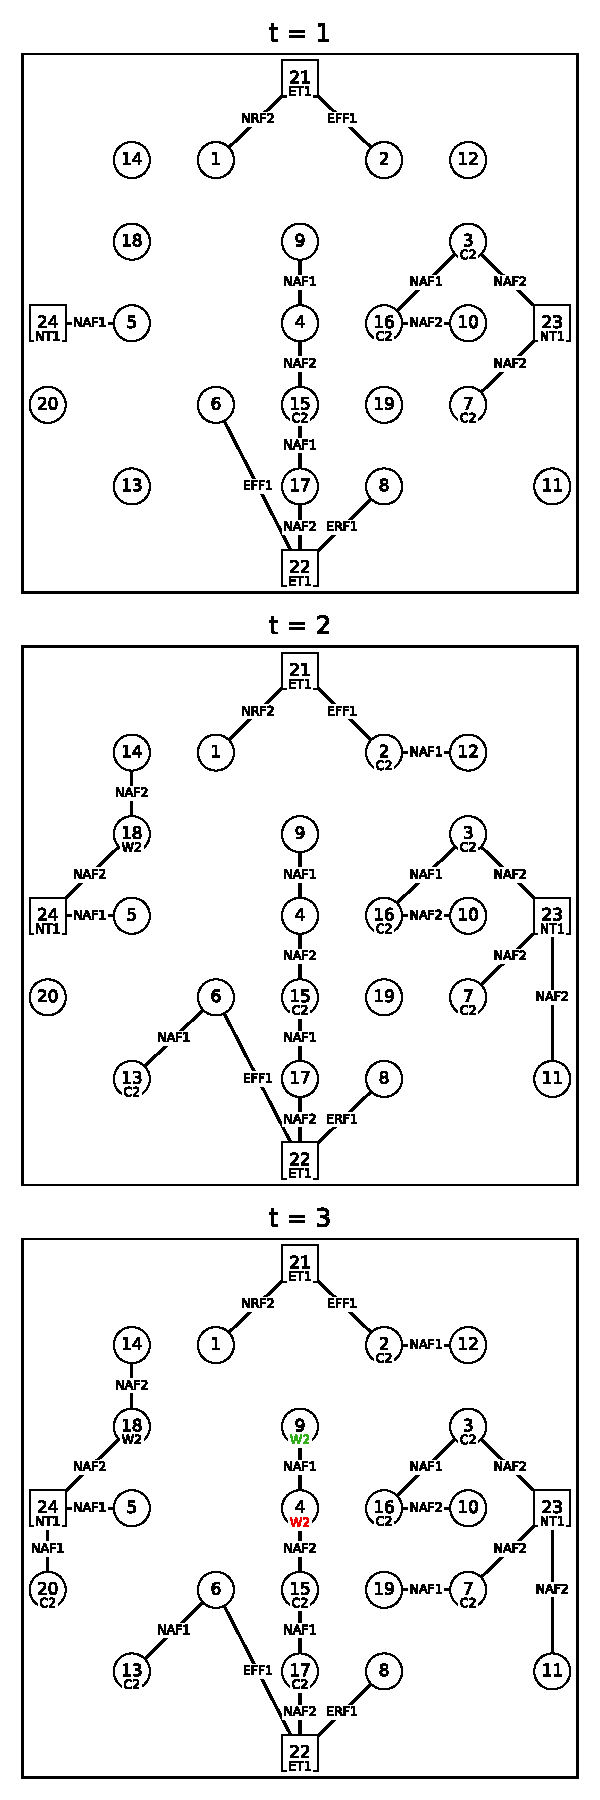
\includegraphics[width=0.5\textwidth]{cap4/resultados/24_gen2.pdf}\\
    \label{fig:24_gen}
\end{figure}

\subsection{Resultados para o sistema de 24 nós -- Apenas veículos elétricos ou cargas}

Neste cenário foram selecionadas quatro soluções (solução 1, 4, 5 e 9) das nove encontradas para serem avaliadas. Estas soluções foram escolhidas pois representam as maiores diferenças entre os valores de \ac{HC} e $c^{TPV}$.

Na figura \ref{fig:24_ev1_4}, é possível observar o que causou a diferença entre a solução 1 (1,3 MVA e 251,62 milhões de dólares) e a solução 4 (0,715 MVA e 251,34 milhões de dólares). Observa-se que esta diferença ocorre devido ao tipo de transformador utilizado em cada solução no nó 23. A solução 1 utiliza a alternativa 2 (um transformador de 15 MVA), já a solução 4 utiliza a alternativa 1 (um transformador de 12 MVA).

Note que mesmo com 3 MVA de capacidade do transformador instalado, a diferença entre os valores de \ac{HC} não foi 3 MVA. Isto ocorre, devido aos limites operacionais de tensão e carregamento do sistema e não apenas devido aos limites de capacidade do transformador e das linhas.  Isto demonstra que estes limites operacionais podem ser violados caso uma carga maior que as encontradas no valor de \ac{HC} deste cenário for instalada no sistema.

Outra característica importante é que não foram observadas mudanças de topologia entre estas duas soluções. O que evidencia que a escolha de transformadores causa um maior impacto no valor de \ac{HC} neste cenário do que mudanças topológicas.

Já na figura \ref{fig:24_ev5_9}, é possível observar o que causou a diferença entre a solução 5 (0,66 MVA e 250,63 milhões de dólares) e a solução 9 (0,12 MVA e 250,3 milhões de dólares). Nestas soluções já observam-se mudanças topológicas significativas, porém, também  observam-se diferentes alternativas de transformadores nó 23, bem como o estágio  de instalação de geradores distribuídos nos nós 2 e 15.

Curiosamente, entre a solução 1 (de maior \ac{HC} e maior $c^{TPV}$) e a solução 9 (de menor \ac{HC} e menor $c^{TPV}$), não há nenhuma diferença topológica. Entretanto, há diferença na construção de uma nova subestação com a instalação de um novo transformador no nó 22 e a alternativa da linha que liga os nós 15 e 17. Isto novamente evidencia que a escolha das alternativas de investimento tem um maior impacto do que a topologia do sistema.

\newpage
\begin{figure}[H]
 	\centering
    \caption{24 nós -- Solução 1 e 4 para o caso de apenas EV. Em vermelho: apenas solução 1. Em verde: apenas solução 4.}
    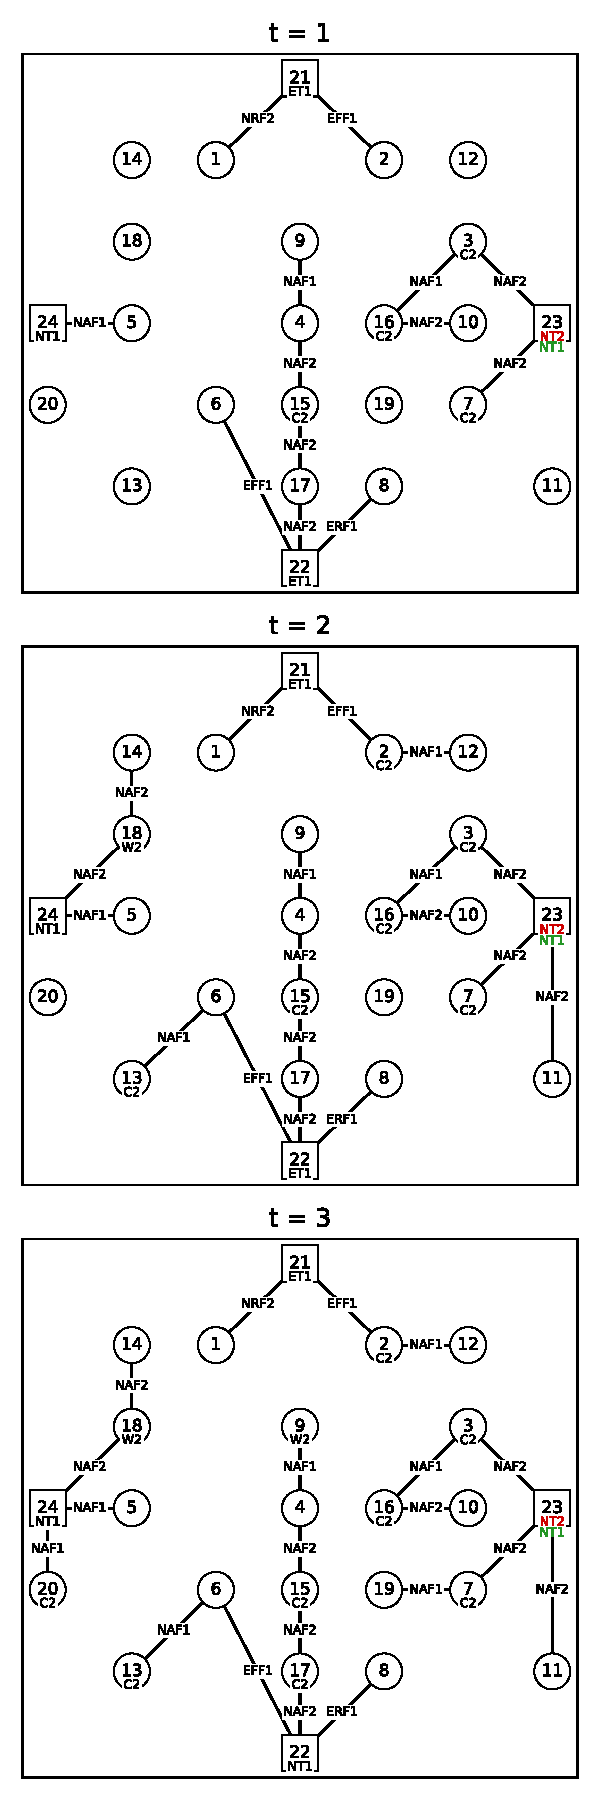
\includegraphics[width=0.5\textwidth]{cap4/resultados/24_ev1.pdf}\\
    \label{fig:24_ev1_4}
\end{figure}

\begin{figure}[H]%
\centering
\caption{24 nós -- Solução 5 e 9 para o caso de apenas EV. (a) Solução 5. (b) Solução 9.}
\begin{tabular}{cc}
    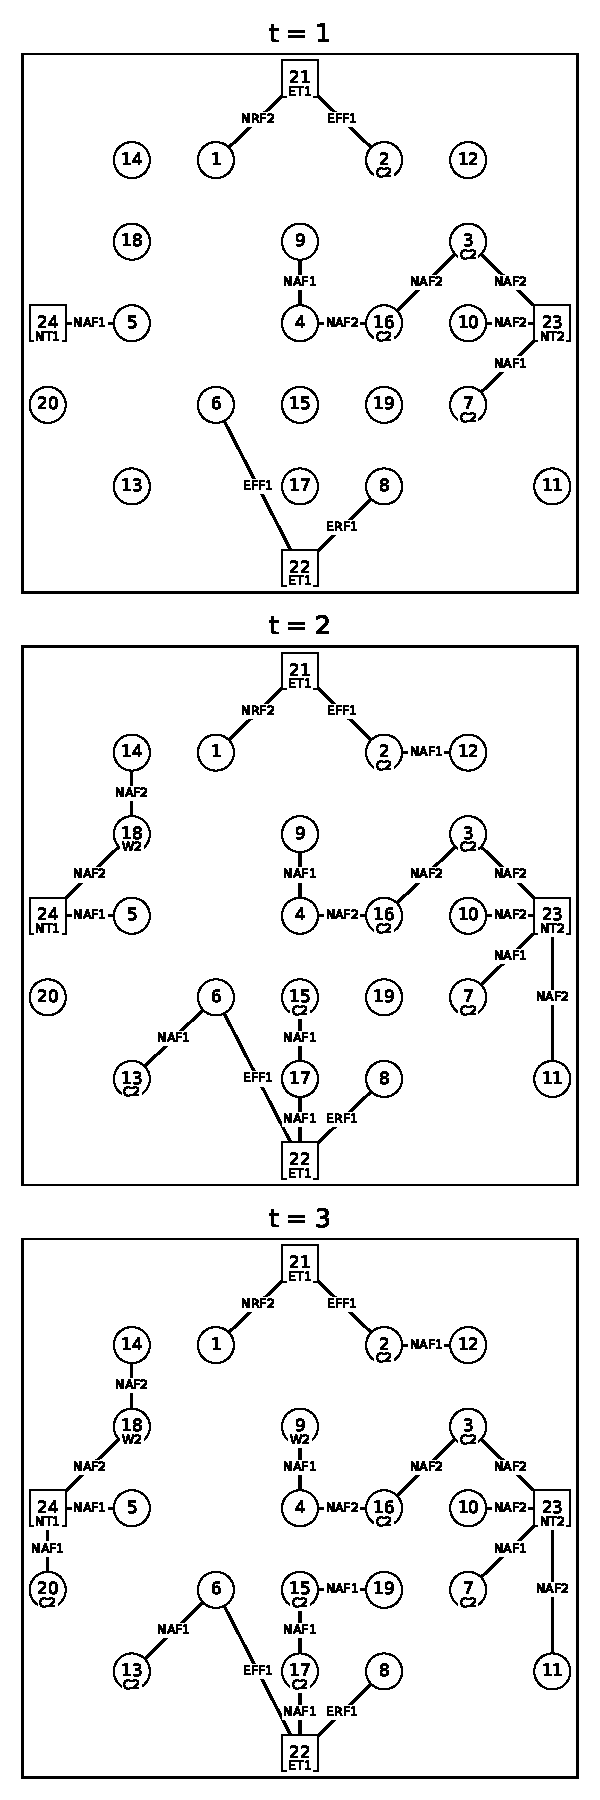
\includegraphics[width=0.49\columnwidth]{cap4/resultados/24_ev5.pdf} & 
    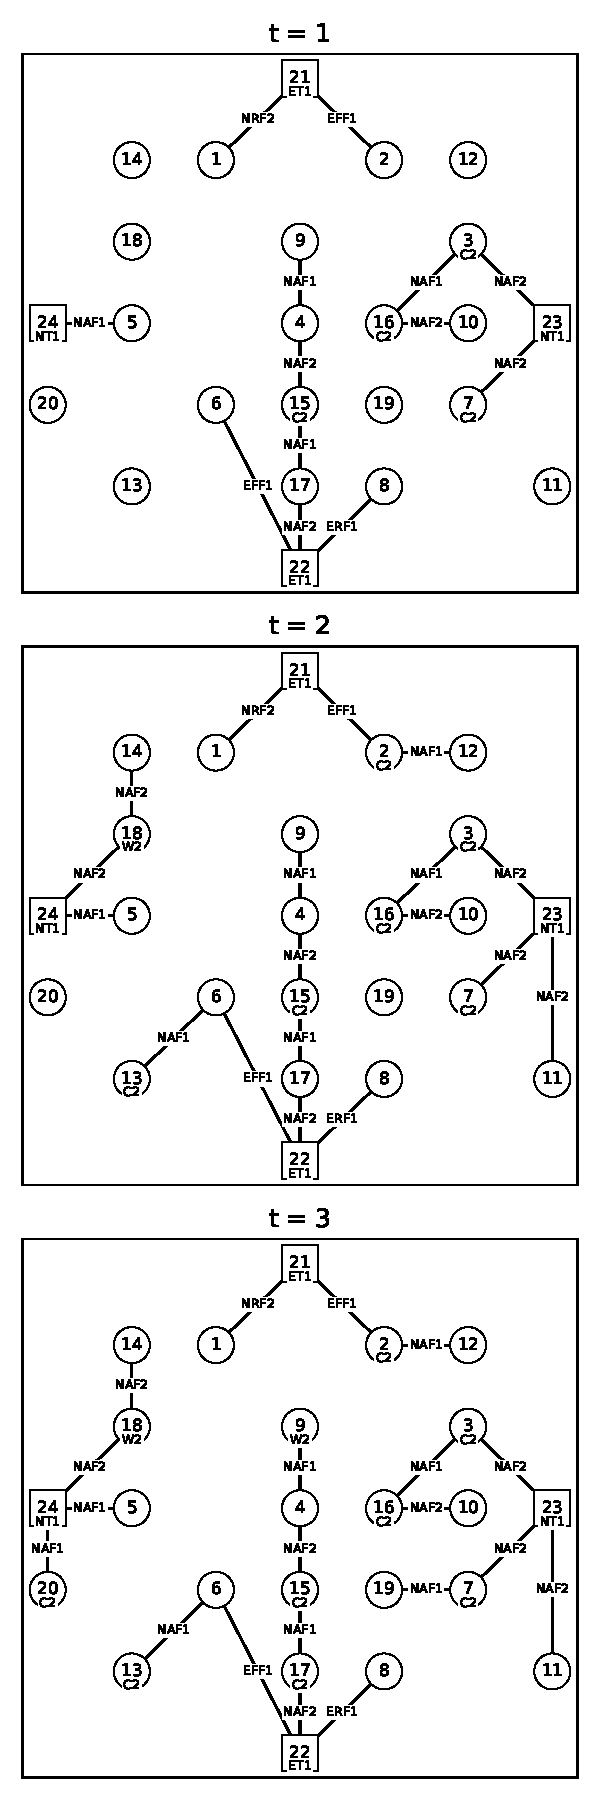
\includegraphics[width=0.49\columnwidth]{cap4/resultados/24_ev9.pdf} \\
    (a) & (b) 
\end{tabular}
\label{fig:24_ev5_9}
\end{figure}

\newpage
\subsection{Resultados para o sistema de 24 nós -- Ambos}

Neste cenário foram selecionadas três soluções (solução 1, 6 e 9) das nove encontradas para serem avaliadas. Estas soluções foram escolhidas pois representam as maiores diferenças entre os valores de \ac{HC} e $c^{TPV}$.


Na figura \ref{fig:24_both1_6} são apresentadas as soluções 1 (784 kVA e 251,65 milhões de dólares) e 6 (452,2 kVA e 250,61 milhões de dólares). Já na figura \ref{fig:24_both9} é apresentada a solução 9 (120 kVA e 250,3 milhões de dólares).

Observa-se uma grande diferença topológica entre as soluções 1 e 6, mas não entre 1 e 9. Indicando mais uma vez que neste sistema mudanças de topologias causam impactos menores, tanto no valor de \ac{HC} quanto nos custos do \ac{PESD}. Curiosamente, há uma grande diferença topológica entre as soluções 6 e 9 também, indicando que mudanças topológicas atuam como um ajuste fino nas soluções encontradas.

Por outro lado, observa-se também grandes diferenças nas opções de investimentos em todas as três soluções apresentadas. Destaca-se a localização do gerador eólico nos nós 4 e 9 nas soluções 1 e 9, bem como a construção de uma nova subestação no nó 22 com a instalação de um novo transformador nas mesmas soluções 1 e 9.

\subsection{Análise entre cenários para o sistema de 24 nós}

Pode-se observar que as diferenças topológicas não impactam tanto quanto as diferenças entre opções de investimentos, principalmente nas soluções em que há diferenças na instalação ou não de novos transformadores e construção de subestações. Entretanto, as soluções observadas neste sistema apresentam fortes evidências que as mudanças topológicas se comportam como um ajuste fino da localização da solução na fronteira de Pareto.

Foi observado também que há um impacto considerável no valor de \ac{HC} dependendo da localização de geradores distribuídos renováveis. Porém, esta localização pouco impacta nos custos do \ac{PESD}. Logo, uma análise mais profunda da localização e da operação destes geradores podem trazer benefícios consideráveis para o valor de \ac{HC} do sistema de distribuição.

Observou-se também que mesmo obtendo-se poucas soluções para o cenário de apenas geradores distribuídos, estas soluções apresentam uma seleção de alternativas e topologia muito semelhante às que são observadas nos outros cenários. O que indica que quanto mais soluções são observadas no cenário apenas de geradores distribuídos, muito mais soluções podem ser observadas nos outros cenários de análise.

\newpage
\begin{figure}[H]%
\centering
\caption{24 nós -- Solução 1 e 6 para o caso de ambos. (a) Solução 1. (b) Solução 6.}
\begin{tabular}{cc}
    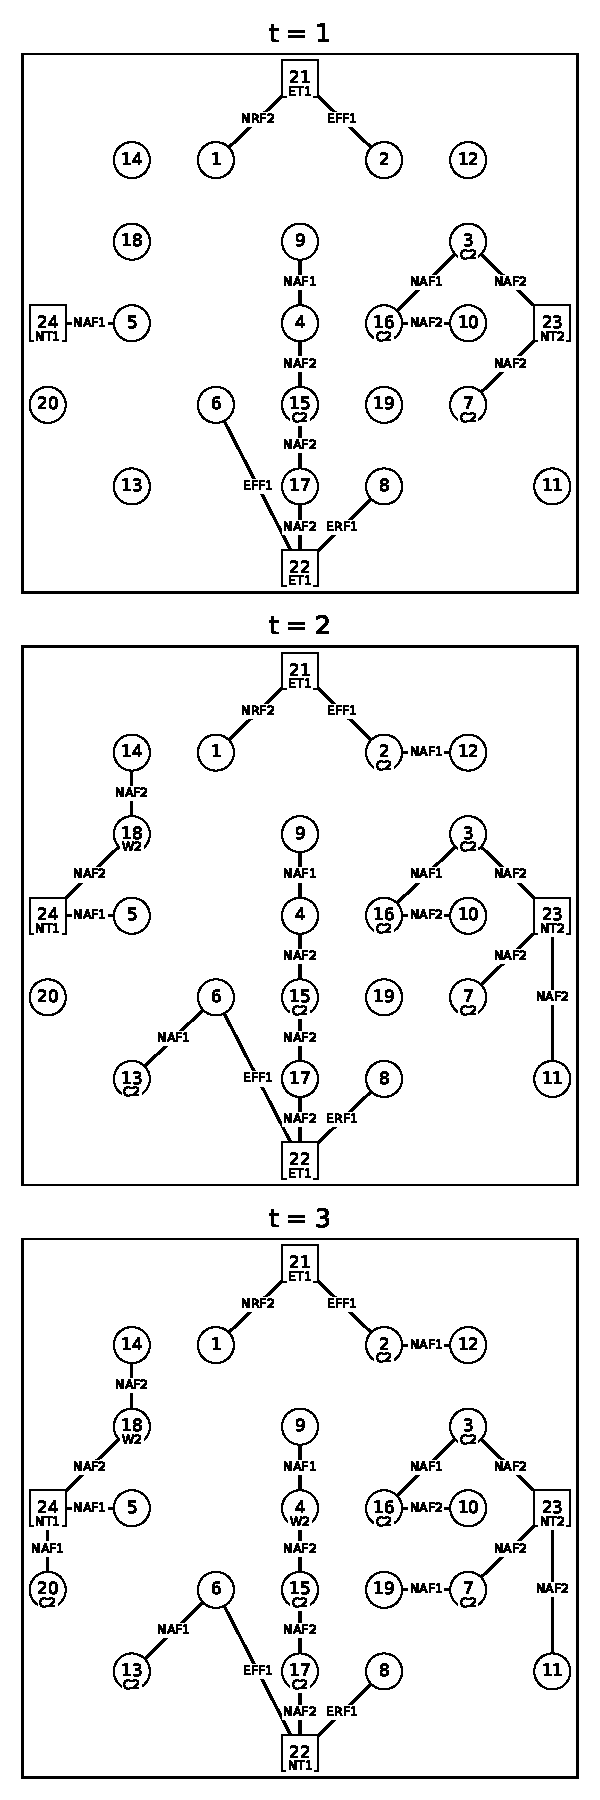
\includegraphics[width=0.49\columnwidth]{cap4/resultados/24_both1.pdf} & 
    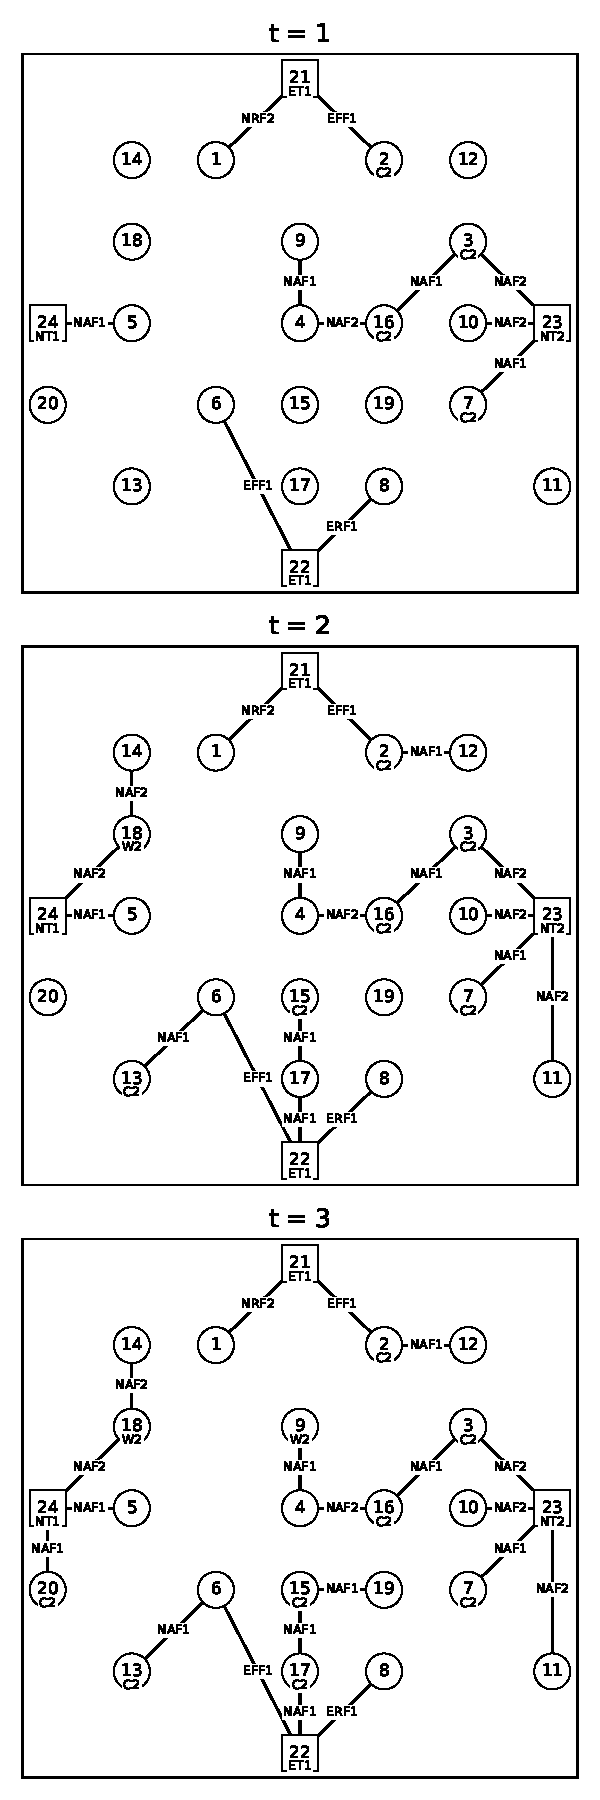
\includegraphics[width=0.49\columnwidth]{cap4/resultados/24_both6.pdf} \\
    (a) & (b) 
\end{tabular}
\label{fig:24_both1_6}
\end{figure}

\begin{figure}[H]
 	\centering
    \caption{24 nós -- Solução 9 para o caso de ambos.}
    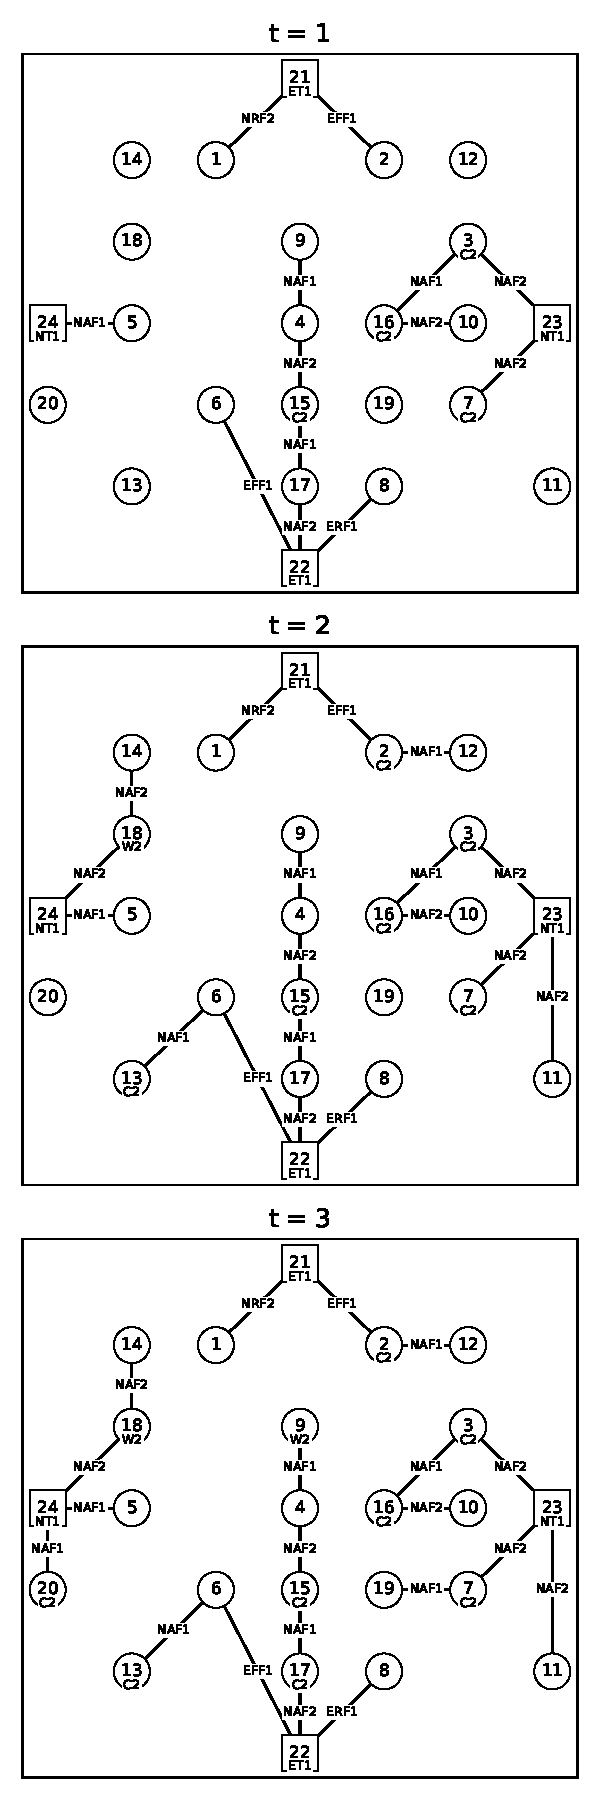
\includegraphics[width=0.5\textwidth]{cap4/resultados/24_both9.pdf}\\
    \label{fig:24_both9}
\end{figure}

\section{Resultados para o sistema de 54 nós}

Para o sistema de 54 nós, também foram realizados três cenários de análise, o primeiro considerando apenas o \ac{HC} para geração distribuída, o segundo considerando o \ac{HC} apenas para veículos elétricos ou novas cargas e o terceiro considerando ambos. Estes cenários foram avaliados com a alteração dos parâmetros $\alpha^{HC}$.

Ao executar a resolução do modelo bi-objetivo para apenas geração distribuída, obteve-se apenas uma solução, com valor de 128,8 kVA de \ac{HC} e 450,86 milhões de dólares de $c^{TPV}$. Por outro lado, tanto para apenas veículos elétricos ou novas cargas quanto para ambos (veículos elétricos e geradores distribuídos), foram obtidas quatro soluções entre 67,8 kVA a 32,3 kVA de \ac{HC} e 458,24 milhões de dólares a 450,86 milhões de dólares de $c^{TPV}$. A figura \ref{fig:54_pareto} apresenta as soluções obtidas, as opções de investimentos podem ser vistas também no Apêndice \ref{sec:tab54}. Vale salientar que o cenário de apenas veículos elétricos ou novas cargas e o cenário para ambos (geração distribuída e veículos elétricos ou novas cargas) apresentaram as mesmas soluções, tanto de investimentos quanto de topologia do sistema.
\vspace{-0.5cm}
\begin{figure}[h]
 	\centering
    \caption{54 nós -- Soluções encontradas.}
    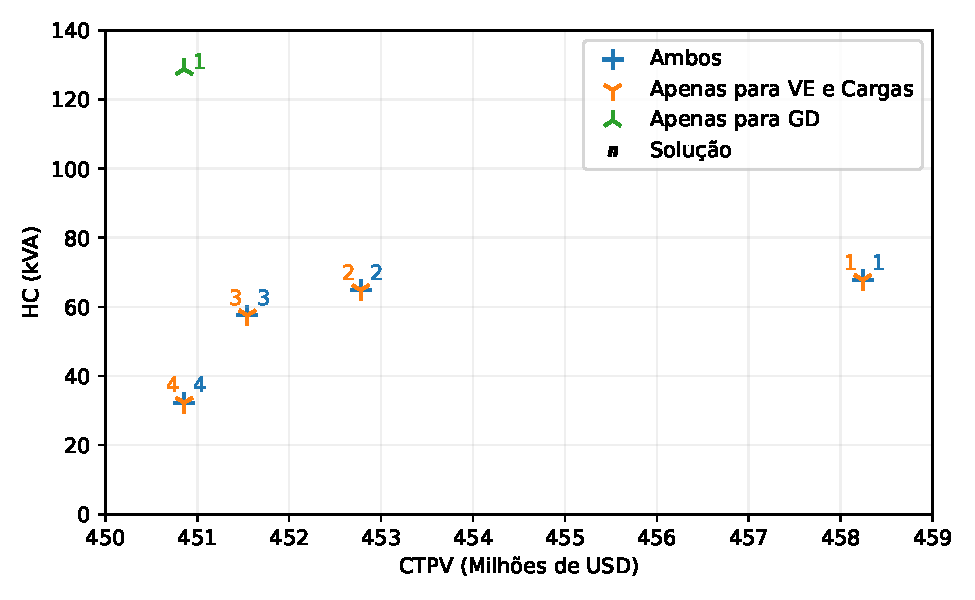
\includegraphics[width=0.8\textwidth]{cap4/resultados/54_pareto.pdf}\\
    \label{fig:54_pareto}
\end{figure}
\vspace{-0.8cm}

É possível observar o mesmo comportamento das soluções de uma relação direta entre o custo total do \ac{PESD} com o valor de \ac{HC} estimado para o sistema. Observa-se também uma relação de aproximadamente 4,81 kVA por milhão de dólares (no caso de ambos), um valor muito menor do qual foi encontrado do sistema de 24 nós, indicando que cada sistema de distribuição a ser planejado possui suas próprias características, porém, seguindo um mesmo comportamento de solução. 


Novamente foi observada uma discrepância de quantidades de soluções entre o cenário de apenas geradores distribuídos e os outros. Novamente, foram testadas alterações no valor de pico das cargas e valores de cenários de carregamentos, porém, não foi encontrada nenhuma evidência que essas alterações impactaram diretamente a diferença de soluções entre os cenários avaliados.

\subsection{Resultados para o sistema de 54 nós -- Apenas geração distribuída}
\vspace{-0.2cm}
Como foram obtidas apenas uma solução para o caso de apenas geração distribuída, facilmente pode-se avaliá-la. Na figura \ref{fig:54_gen}, observa-se que todas as barras que podem receber geradores distribuídos, foram instalados geradores distribuídos, inclusive, mais de um gerador distribuído por nó como, por exemplo, no nó 15, no qual foi instalado um gerador eólico e um gerador convencional. Isto indica que a solução encontrada busca manter controlada a operação do sistema de distribuição, pois apenas os geradores convencionais possuem a capacidade de controle de despacho.
Observa-se também que mesmo com todos os geradores instalados, novas subestações foram necessárias e que isso não causou tantos impactos no valor final de $c^{TPV}$ em relação às soluções encontradas nos outros cenários.
\vspace{-0.2cm}
\begin{figure}[H]
 	\centering
    \caption{54 nós -- Solução 1 para o caso de apenas geração.}
    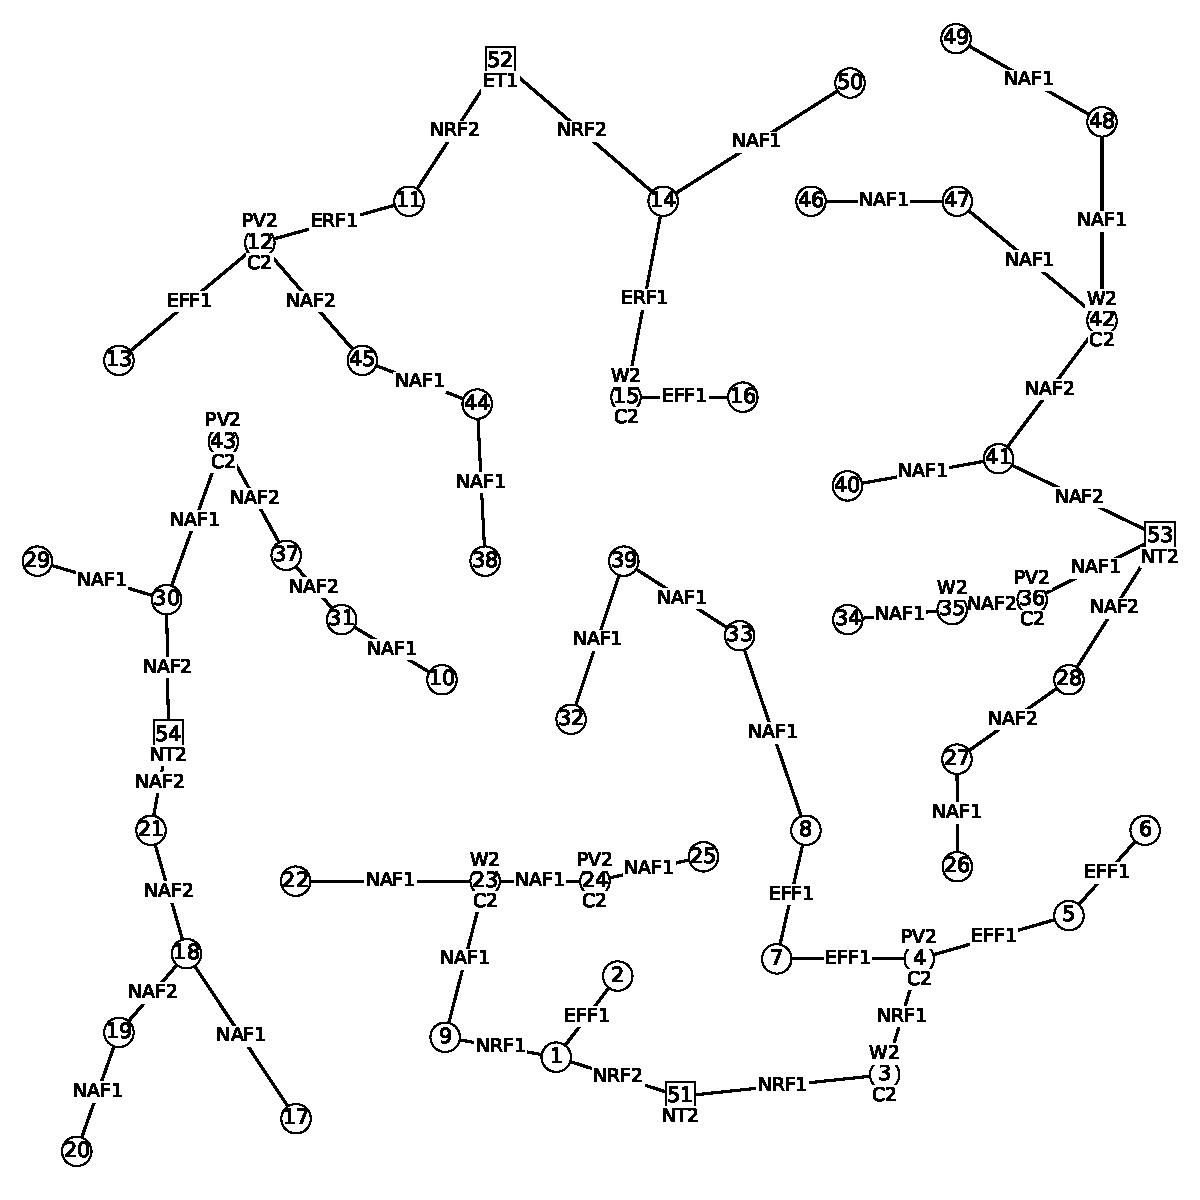
\includegraphics[width=1.02\textwidth]{cap4/resultados/54_bus_gen.pdf}\\
    \label{fig:54_gen}
\end{figure}


\subsection{Resultados para o sistema de 54 nós -- Ambos e apenas veículos elétricos ou cargas}

Como o cenários de ambos e apenas veículos elétricos ou cargas apresentaram as mesmas soluções, elas são apresentadas juntas nas figuras de \ref{fig:54_both1} a \ref{fig:54_both4}.

Observa-se na solução 1 (figura \ref{fig:54_both1}) que todos os nós que podem ter geradores distribuídos instalados, tiveram geradores instalados e que os mesmos geradores, subestações e transformadores foram instalados da mesma forma que a solução para apenas geração distribuída. Por outro lado, há uma diferença significativa na topologia do sistema de distribuição, isso ocorre devido a presença das novas cargas no sistema de distribuição no cenário de ambos e apenas veículos elétricos ou cargas que não ocorrem no cenário de apenas geradores elétricos.

\begin{figure}[h]
 	\centering
    \caption{54 nós -- Solução 1 para o caso de ambos e apenas veículos elétricos ou cargas.}
    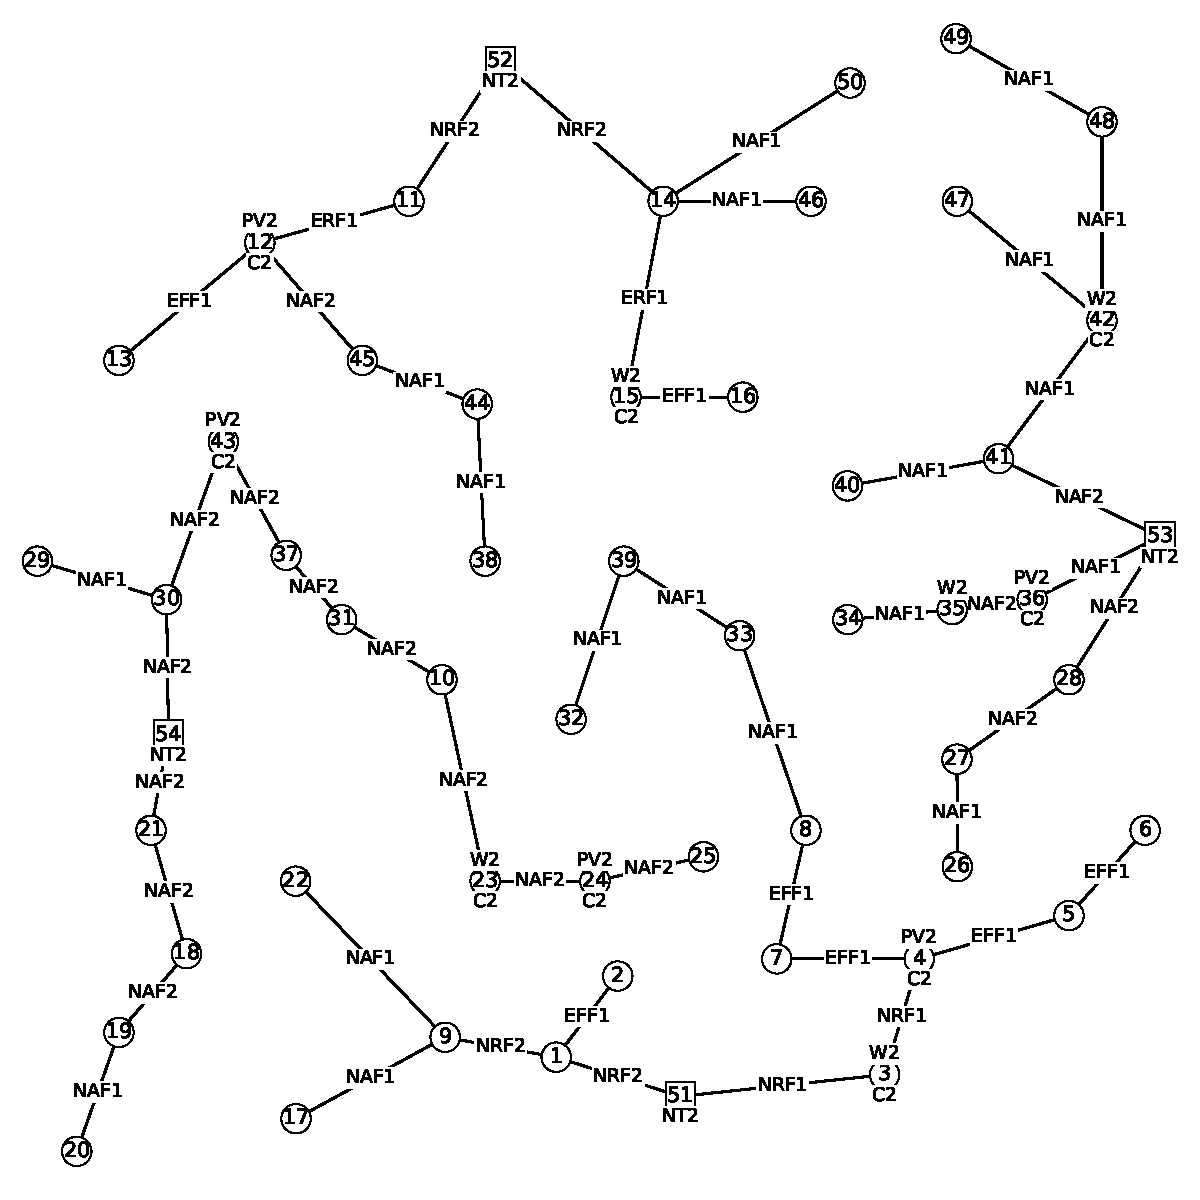
\includegraphics[width=1.02\textwidth]{cap4/resultados/54_bus_both1.pdf}\\
    \label{fig:54_both1}
\end{figure}


Já na solução 2 (figura \ref{fig:54_both2}) observou-se também que todos os nós que podem ter geradores tiveram estes instalados da mesma forma que as outras soluções apresentadas anteriormente. Por outro lado, com uma diferença significativa na topologia do sistema de distribuição. Curiosamente, apenas a topologia e a operação dos geradores convencionais foram diferentes entre as duas soluções. Este comportamento é observado também na solução 3 (figura \ref{fig:54_both3}), que não apresenta diferença entre os investimentos que não sejam relacionados a topologia e cabos de alimentadores.
\begin{figure}[h]
 	\centering
    \caption{54 nós -- Solução 2 para o caso de ambos e apenas veículos elétricos ou cargas.}
    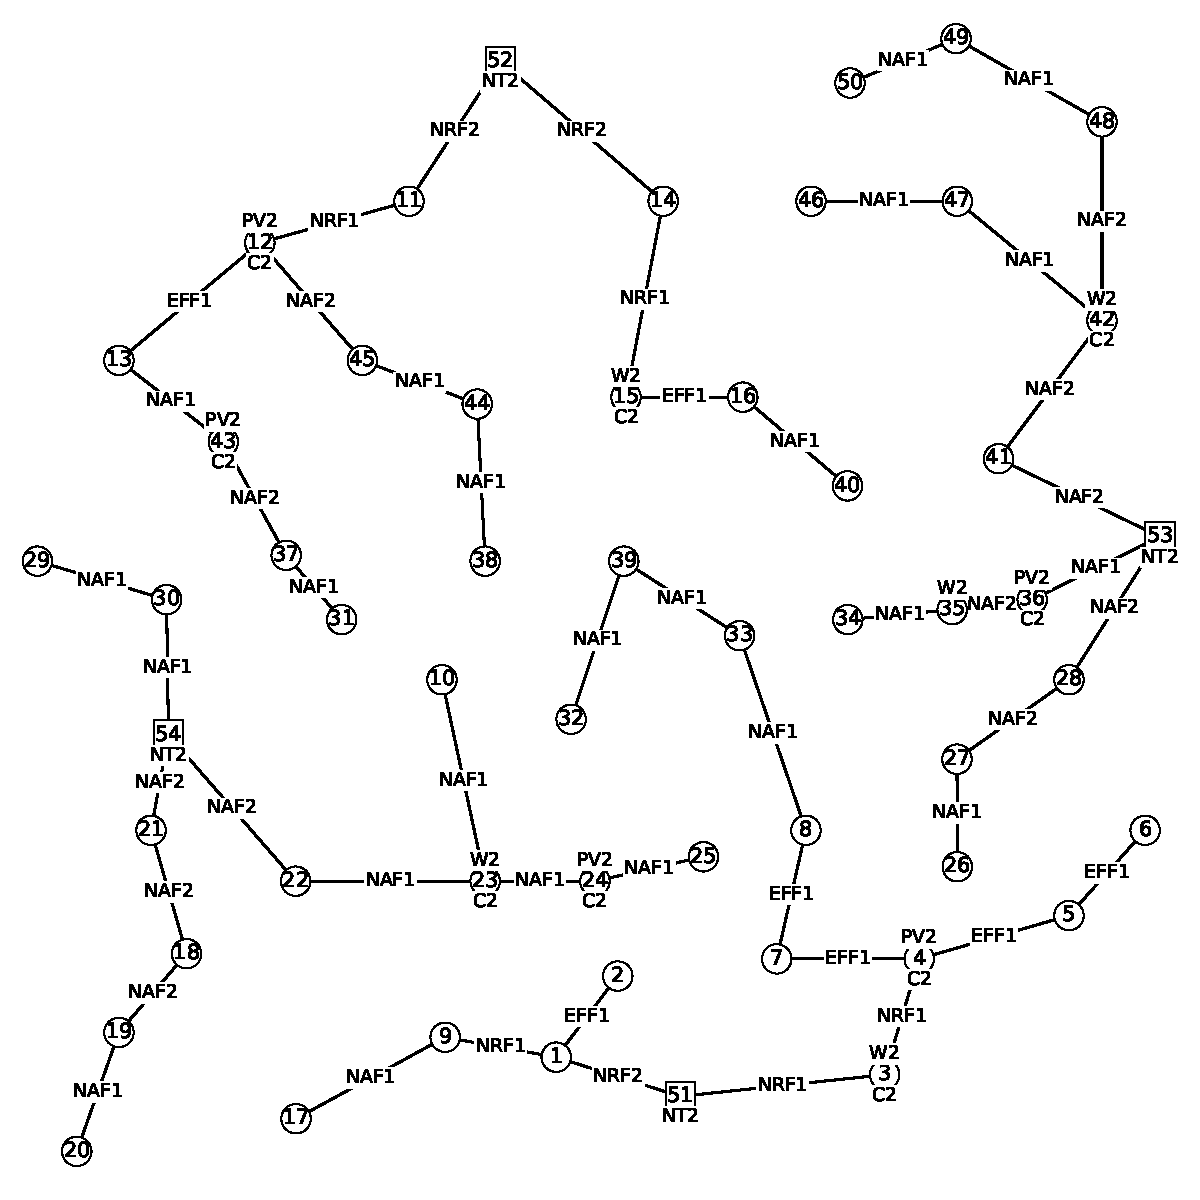
\includegraphics[width=1.02\textwidth]{cap4/resultados/54_bus_both2.pdf}\\
    \label{fig:54_both2}
\end{figure}

\begin{figure}[ht]
 	\centering
    \caption{54 nós -- Solução 3 para o caso de ambos e apenas veículos elétricos ou cargas.}
    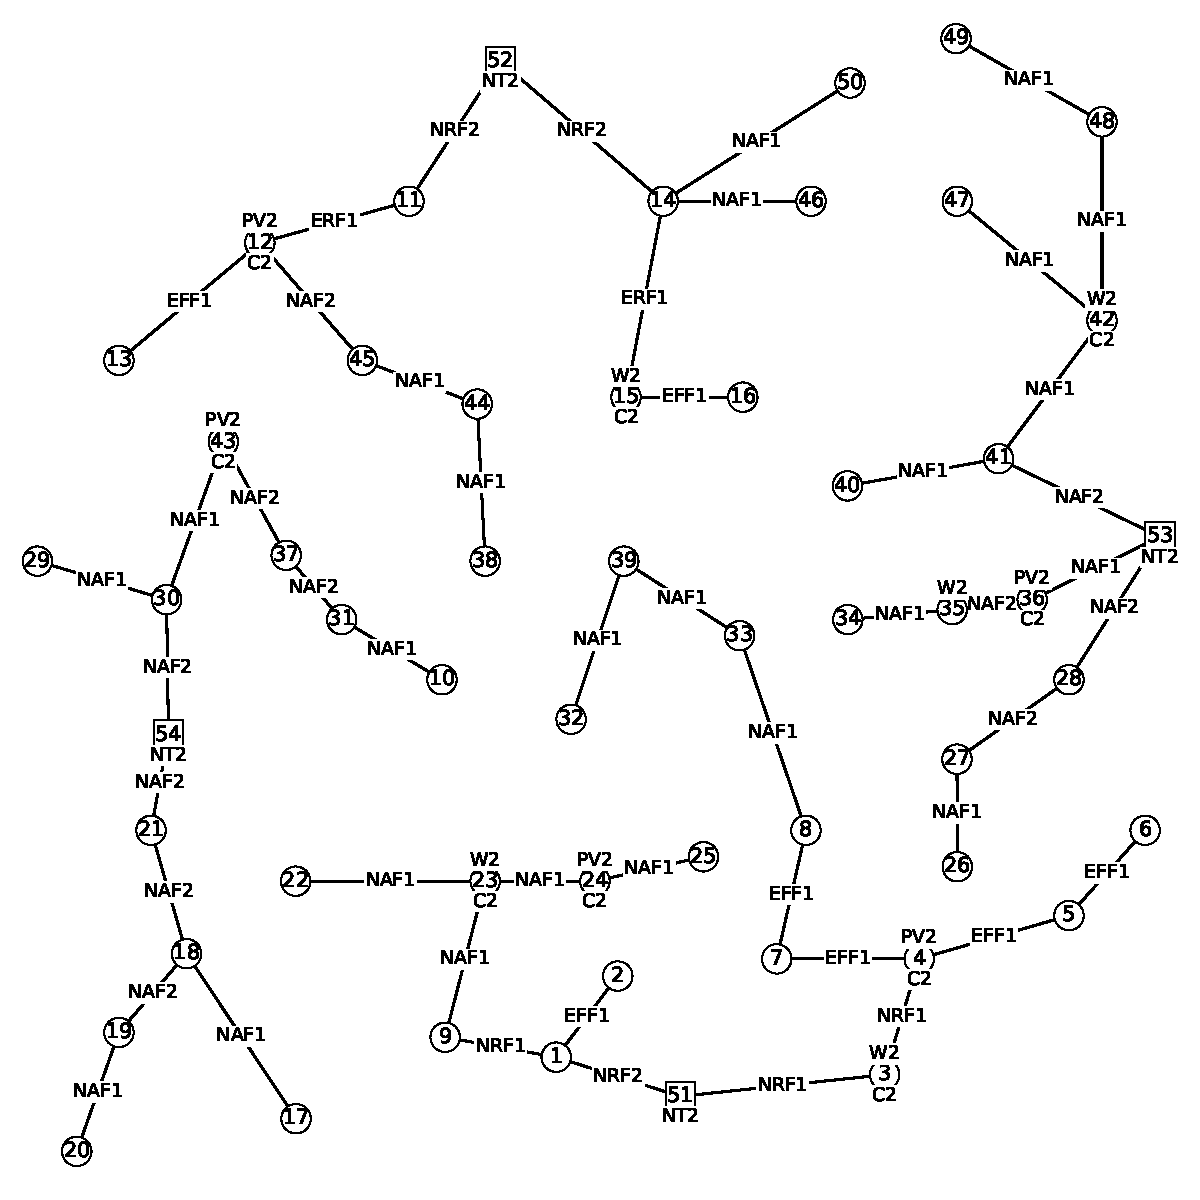
\includegraphics[width=1.02\textwidth]{cap4/resultados/54_bus_both3.pdf}\\
    \label{fig:54_both3}
\end{figure}

Observa-se, porém, que na solução 4 (figura \ref{fig:54_both4}) há uma diferença nas opções de investimentos que não a topologia/cabos. Nesta solução, não foi feito o investimento de construção da subestação e instalação de um novo transformador nó 52, o que impactou diretamente os valores de \ac{HC} e $c^{TPV}$. 

\subsection{Análise entre cenários para o sistema de 54 nós}

Diferente do que foi observado no sistema de 24 nós, neste, ocorreu um impacto significativo da topologia do sistema, visto que não foram encontradas outras soluções com outras opções de investimentos que poderiam gerar uma solução dominante durante as buscas dos pontos da fronteira de Pareto. Entretanto, as soluções encontradas para este sistema também indicam que o ajuste da topologia do sistema de distribuição se comporta como um ajuste fino dos pontos na fronteira de Pareto, visto que a mudança de transformador no nó 52 causa um grande impacto, tanto no valor de \ac{HC} quanto no valor de $c^{TPV}$.

Observou-se também, que nós com geradores renováveis também tiveram geradores convencionais instalados nos mesmos. Isto pode indicar que este sistema precisa de uma certa "estabilidade"\; na geração distribuída para manter os níveis de tensão adequados, bem como a capacidade de \ac{HC}.

Por fim, destaca-se a diferença de valor de \ac{HC} entre a solução para apenas geradores distribuídos e as soluções para ambos e apenas veículos elétricos ou cargas. Isto indica que este sistema é muito mais receptivo a instalação de novos geradores distribuídos do que novas cargas.

\begin{figure}[h]
 	\centering
    \caption{54 nós -- Solução 4 para o caso de ambos e apenas veículos elétricos ou cargas.}
    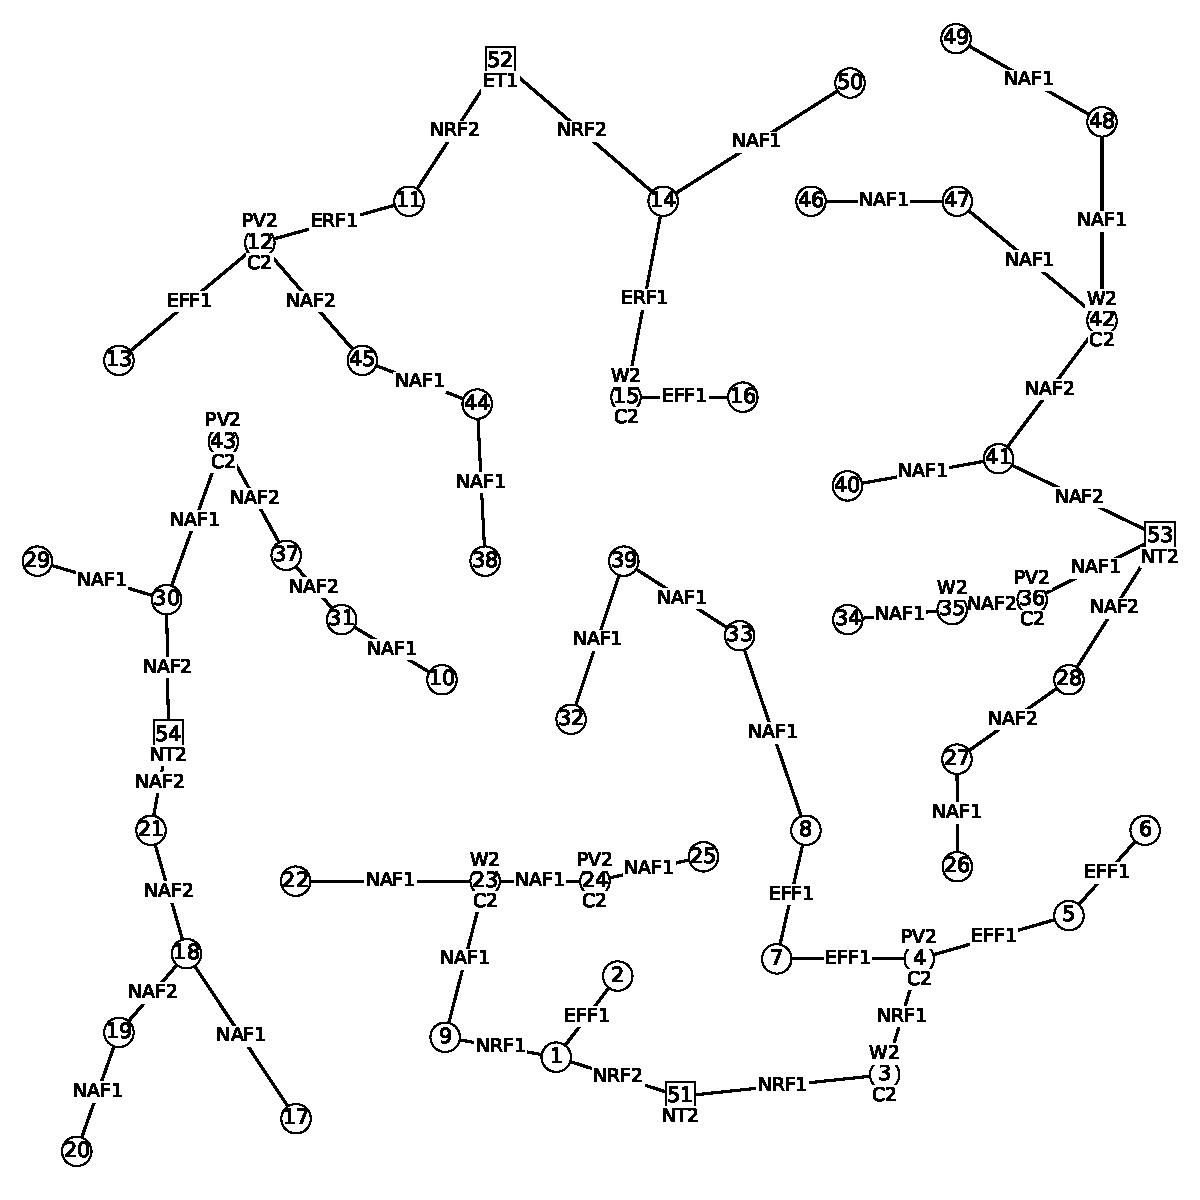
\includegraphics[width=1.02\textwidth]{cap4/resultados/54_bus_both4.pdf}\\
    \label{fig:54_both4}
\end{figure}

\newpage
\section{Resultados para o sistema de 138 nós}

Para o sistema de 138 nós, também foram realizados três cenários de análise, o primeiro considerando apenas o \ac{HC} para geração distribuída, o segundo considerando o \ac{HC} apenas para veículos elétricos ou novas cargas e o terceiro considerando ambos. Estes cenários foram avaliados com a alteração dos parâmetros $\alpha^{HC}$.

Diferente de todos os outros resultados obtidos, no sistema de 138 nós, foram encontradas 10 soluções para caso de apenas geração distribuída, 44 soluções para o caso de apenas veículos elétricos ou novas cargas e 34 soluções para o caso de ambos. Todas as opções de investimentos podem ser vistas no Apêndice \ref{sec:tab54}, as soluções foram enumeradas de forma que a solução com menor índice indica maior \ac{HC} e a solução com maior índice indica menor \ac{HC}, conforme a implementação apresentada na figura \ref{fig:method}.

A figura  \ref{fig:54_pareto} apresenta os pontos da fronteira de Pareto obtidas durante a resolução do modelo bi-objetivo em todos os três cenários de análise. Note que para o cenário de apenas geração distribuída o \ac{HC} varia entre 78,055 kVA ($c^{TPV}$ de 118,94 milhões de dólares) e  17,815 kVA ( $c^{TPV}$ de 117,07 milhões de dólares). Já para o caso de apenas veículos elétricos ou novas cargas o \ac{HC} varia entre 118,555 kVA ($c^{TPV}$ de 120,52 milhões de dólares) e 7,141 kVA ($c^{TPV}$ de 117,07 milhões de dólares). No caso de ambos o \ac{HC} varia entre 68,905 kVA ($c^{TPV}$ de 122,35 milhões de dólares) e 7,143 kVA ($c^{TPV}$ de 117,07 milhões de dólares).

\begin{figure}[h]
 	\centering
    \caption{138 nós -- Soluções encontradas.}
    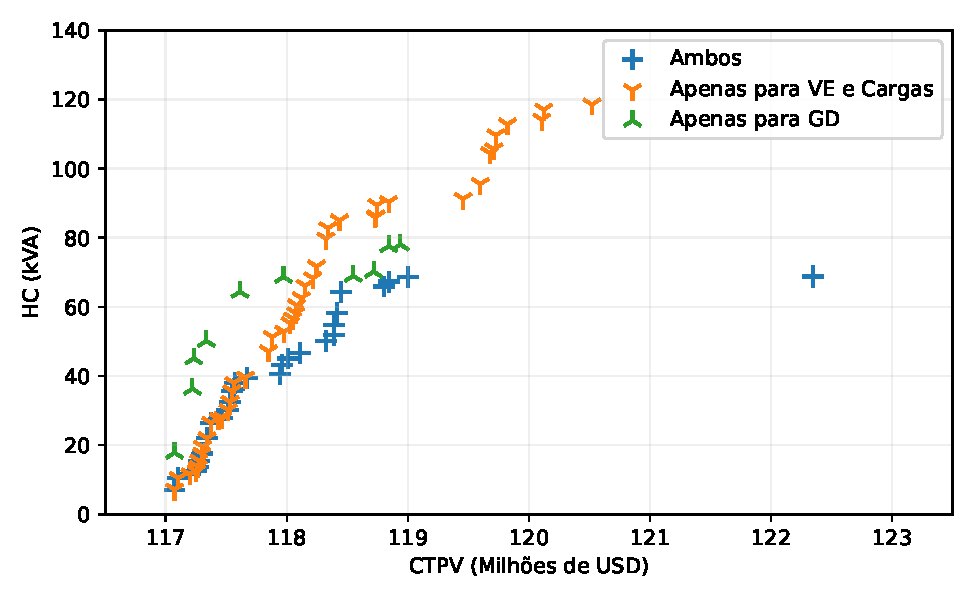
\includegraphics[width=0.8\textwidth]{cap4/resultados/138_pareto.pdf}\\
    \label{fig:138_pareto}
\end{figure}

É possível observar o mesmo comportamento das soluções de uma relação direta entre o custo total do \ac{PESD} com o valor de \ac{HC} estimado para o sistema. Observa-se também uma relação de aproximadamente 11,69 kVA por milhão de dólares, um valor muito menor do qual foi encontrado do sistema de 24 nós, porém na mesma magnitude do sistema de 54 nós. Isto reforça a hipótese de que cada sistema de distribuição a ser planejado possui suas próprias características, porém, seguindo um mesmo comportamento de solução. 

Apesar de ter sido obtido mais soluções para o caso de apenas geradores distribuídos, a mesma discrepância de quantidades de soluções entre o cenário de apenas geradores distribuídos e os outros foi observada. Novamente, foram testadas alterações no valor de pico das cargas e valores de cenários de carregamentos, porém, não foi encontrada nenhuma evidência que essas alterações impactaram diretamente a diferença de soluções entre os cenários avaliados.

Durante a escrita desta tese, não foi identificado uma boa forma de representar graficamente todas as diferenças entre as soluções e ainda assim apresentar o sistema final obtido através das soluções de investimentos encontradas em sistemas de distribuição grandes como o de 138 nós. Exemplos de trabalhos similares também sofrem do mesmo problema. Desta forma, a discussão dos resultados é apresentada pontuando investimentos e mudanças de topologias relevantes identificadas nas soluções. Caso seja necessário mais detalhes sobre as soluções, o autor indica a inspeção das tabelas no Apêndice \ref{sec:tab54} e o código fonte implementado, disponível em \cite{modelocomHC}.

\subsection{Resultados para o sistema de 138 nós -- Apenas geração distribuída}

No sistema de 138 nós observou-se que a melhoria de \ac{HC} ocorre através da instalação de geradores distribuídos e da topologia do sistema de distribuição. Não houve alterações nas opções de transformadores, nem a construção de novas subestações, sendo a construção da subestação e a instalação de transformador nos nós 138, 137 e 136 foram necessárias em todas as soluções encontradas.

Com relação a diferença de geradores distribuídos, a diferença entra a solução com maior \ac{HC} (solução 1) e a solução com menor \ac{HC} (solução 10) se dá pela alternativa de investimento nos geradores distribuídos convencionais dos nós 94 e 53 e pela instalação ou não de um gerador eólico (alternativa 2) no nó 52. Nos nós 94 e 53, a solução 1 opta por instalar geradores distribuídos convencionais com maior potência (alternativa 2) do que a solução 10. Já a solução 10 opta por instalar o gerador eólico no nó 52. Isto pode indicar que a operação dos geradores convencionais de maior capacidade trazem maior flexibilidade na operação, possibilitando um maior valor de \ac{HC}, enquanto a inserção de geradores renováveis sem um devido controle de sua operação pode prejudicar o valor de \ac{HC}, mesmo que reduzam os custos de operação.

Já analisando a mudança topológica entre a solução com maior \ac{HC} (solução 1) e a solução com menor \ac{HC} (solução 10), é possível observar que são sistemas diferentes, mas que possuem semelhanças. Isso é observado já que apenas quatro alimentadores são diferentes entre as soluções. A solução 1 interliga os nós: 104 ao 105, 44 ao 45, 111 ao 112, 114 ao 123, todos utilizando a alternativa 1. A solução 10 interliga os nós: 43 ao 52, 28 ao 29, 108 ao 138, 113 ao 114, todos utilizando a alternativa 1.

Durante a avaliação das soluções, foi observado apenas um caso em que a escolha de um condutor com mais ampacidade resultou em uma mudança de valor de \ac{HC}. Isto ocorre na diferença entre as soluções 7 e 8 no alimentador que interliga o nó 43 ao 52. Entretanto, a diferença entre as duas soluções também apresenta diferenças entre instalação de geradores convencionais e de topologia do sistema planejado.

De modo geral, observou-se que os geradores despacháveis melhoraram o valor de \ac{HC} neste sistema com este cenário de análise, bem como mudanças topológicas.

\subsection{Resultados para o sistema de 138 nós -- Apenas veículos elétricos e cargas}

No caso de apenas veículos elétricos e cargas as diferenças são mais evidentes, pois há tanto instalação geradores distribuídos diferentes, topologias diferentes, construção de novas subestações, instalação de novos transformadores e instalação de condutores com maior ampacidade.

Em relação aos geradores distribuídos instalados e comparando a solução com maior \ac{HC} (solução 1) e a solução com menor \ac{HC} (solução 44), é possível observar que possuem a mesma quantidade de geradores instalados. Porém, a solução 1 instala um gerador convencional com maior potência no nó 94 e outro no nó 133, enquanto a solução 10 instala um gerador convencional com menor potência no nó 94 e um gerador eólico no nó 52.

Destaca-se também a escolha da solução 1 de se construir novas subestações e transformadores nos nós 136 e 137 em relação a não opção pelos mesmos na solução 44. Por fim, vale observar que as topologias também são diferentes, porém com grande semelhanças entre eles, visto que apenas 7 alimentadores são diferentes entre a solução 1 e a solução 44.

Dentre as 44 soluções, pode-se observar que apenas 11 investimentos para aumentar a ampacidade de linhas foram são escolhidos se for avaliado a diferença entre as soluções par a par. A maioria destes investimentos ocorrem no alimentador que liga o nó 105 ao 122. Curiosamente, o observou-se também a escolha de se reduzir a ampacidade de um alimentador (mesmo com melhoria de \ac{HC}), especialmente entre os nós 43 e 52. Esta última observação pode ser explicada pela redução de corrente que flui pelos nós 43 e 52 com a mudança de topologia.

Da mesma forma que anteriormente, observou-se que geradores despacháveis melhoraram o valor de HC neste sistema com este cenário de análise, bem como mudanças topológicas.

\subsection{Resultados para o sistema de 138 nós -- Ambos}

Para o caso de ambos ocorrem as mesmas diferenças observados para o caso de apenas veículos elétricos e cargas, porém, é possível observar mais soluções que apresentam a decisão de aumentar a ampacidade de um dos condutores para elevar o valor de \ac{HC} em relação a solução vizinha. Neste caso de análise, observou-se a instalação de geradores distribuídos diferentes, topologias diferentes, construção de novas subestações, instalação de novos transformadores e instalação de condutores com maior ampacidade.

Da mesma forma que o caso de apenas veículos elétricos e cargas, a solução com maior \ac{HC} (solução 1) apresenta a escolha de mais geradores distribuídos convencionais, enquanto a solução com menor \ac{HC} (solução 34) opta por instalar mais geradores eólicos. Observou-se também a opção de se construir novas subestações e instalar novos transformadores nos nós 136 e 137 na solução 1 que não é observada na solução 34.

A decisão de aumentar a ampacidade das linhas foi mais evidente neste cenário de análise, principalmente nas primeiras soluções. Foi observado que a opção por condutores de maior ampacidade ocorreu como um ajuste ainda mais fino do valor de \ac{HC}, além do ajuste feito pelas mudanças de topologia.

E mais uma vez se observou que geradores despacháveis melhoraram o valor de HC neste sistema com este cenário de análise, bem como mudanças topológicas.



\subsection{Análise entre cenários para o sistema de 138 nós}

Neste sistema foi observado que ocorrem cenários em que mudanças topológicas causam um aumento significativo no valor do \ac{HC} enquanto há cenários em que as outras opções de investimentos causam maiores impactos neste indicador. Como este sistema é maior, levanta-se a hipótese de que quanto maior o sistema, maior a quantidade de soluções que podem ser encontradas na fronteira de Pareto. Por outro lado, é possível que esta quantidade maior de soluções seja possível devido às características topológicas e das opções de investimentos.

Observou-se que os geradores renováveis impactaram negativamente o valor de \ac{HC}. Esta observação pode ser explicada pois no modelo implementado, os geradores renováveis não são despacháveis, o que causa um "consumo" da banda de \ac{HC} disponível em uma determinada solução. Outra hipótese que pode ser levantada é que este sistema precisa de uma certa "estabilidade"\; na geração distribuída para manter os níveis de tensão adequados, bem como a capacidade de \ac{HC}.

Por fim, destaca-se a diferença de valor de \ac{HC} entre a solução para apenas geradores distribuídos e as soluções para ambos e apenas veículos elétricos ou cargas. Isto indica que este sistema é muito mais receptivo a instalação de novas cargas e veículos elétricos.

% \section{Estimativa da capacidade de hospedagem}

% A estimativa do valor de HC do sistema de distribuição é realizada em conjunto com o PESD e os valores de contribuição de cada nó para o valor total do HC em cada estágio pode ser vista na figura \ref{fig:result_hc}.

% Observa-se que o valor de HC vai aumentando com o passar dos estágios e que nem todos os nós do sistema contribuem para o valor de HC. Isto é esperado para os nós que não estão conectados ao sistema de distribuição, por outro lado, no segundo e terceiro estágio os nós 12 e 13 não contribuem para o valor de HC mesmo estando conectados e possuindo cargas. Isto nos leva a crer que há múltiplas soluções dos HC locais, porém o valor total estimado permanece o mesmo. Desta forma, observa-se que a estimativa do HC local não deve ser considerada como rígida, sendo necessário a avaliação do HC a cada solicitação de nova instalação de geradores distribuídos.


% A partir dos resultados de investimentos e custos, no qual foi observado uma grande quantidade de alocação dos geradores distribuídos operados pela empresa distribuidora, esperava-se que isto impactaria no valor de HC estimado. Porém, como estes geradores distribuídos são despacháveis o aumento da injeção de outros geradores distribuídos (estes já não controlados pela empresa distribuidora) são compensados com a redução de injeção de potência dos que já foram instalados. Este comportamento nos leva a perceber que os geradores distribuídos já alocados podem acabar em desuso com o crescimento da injeção de novos geradores distribuídos. 

% Desta forma, observa-se que há um típico comportamento de risco associado à instalação dos geradores distribuídos durante a expansão do sistema de distribuição, que envolve alocá-los para que, em um futuro próximo, talvez sejam subutilizados e não contribuindo para uma redução significativa no valor presente líquido dos custos totais, visto que a maior parte provém da expectativa de menor custos com produção de energia. 

% Por outro lado, a alocação destes geradores distribuídos operados pela empresa distribuidora, fornecem um certa segurança em relação a operação do sistema de distribuição. Visto que é garantido que todos os requisitos operacionais serão atendidos, com ou sem novos geradores distribuídos instalados.

% Vale observar que no modelo utilizado não está prevista a instalação de sistemas de armazenamento de energia, dos quais podem contribuir tanto para a operação do sistema de distribuição, quanto para a melhoria do valor de HC observado nos resultados obtidos.

% Levanta-se o questionamento sobre o HC de estações de veículos elétricos que, do ponto de vista do modelo utilizado, se comportam apenas como novas cargas no sistema de distribuição e poderá ser implementado neste modelo futuramente. Talvez, com a integração destas novas cargas o risco de desuso de geradores distribuídos instalados durante a expansão do sistema de distribuição pode deixar de se tornar relevante, principalmente pelo comportamento de grandes picos e vales na demanda que estas cargas causam.

% Por fim, não é possível deixar de observar que o modelo proposto já indica uma otimização multi-objetivo que relaciona os custos com o PESD com a melhoria do valor de HC. Espera-se que no futuro sejam implementadas rotinas para expressar esta relação. Por outro lado, a integração tanto do HC de estações de veículos elétricos quanto a alocação de sistemas de armazenamento de energia também podem auxiliar na identificação desta relação.
